\RequirePackage{ifpdf}
%\documentclass[notes,handout]{beamer}
\documentclass[notes=false,pdftex]{beamer}
\usepackage[latin1,utf8]{inputenc}
\usepackage[czech]{babel}
\usepackage{multimedia}
\usepackage{listings}
\lstset{
	language=C,
	basicstyle=\small,
	tabsize=2,
	numbers=left,             
	numberstyle=\scriptsize,  
	stepnumber=1,             
	numbersep=10pt            
}

\usetheme{umbc2}
%\useoutertheme{umbcfootline} 

\author{Filip Jareš, Tomáš Juchelka} 
\title{Segmentace polygonální mapy pro multirobotickou exploraci} 
\institute[FEL ČVUT] {
  Katedra kybernetiky\\[2ex]
  Elektrotechnická fakulta\\[2ex]
  České vysoké učení technické\\[2ex]
  \vspace{1ex}
  \texttt{jaresfil@fel.cvut.cz, juchetom@fel.cvut.cz}
  \vspace{1ex}
}
\date{Mobilní a kolektivní robotika (A3M33MKR)\hspace{7ex}18. 1. 2012}

%\setbeamertemplate{items}[ball] 
%\setbeamertemplate{navigation symbols}{} 
%\setbeamertemplate{blocks}[rounded][shadow=true] 
\setbeamercovered{transparent}

\begin{document}

%%%%%%%%%%%%%%%%%%%%%%%%%%%%%%%% Titulní slide %%%%%%%%%%%%%%%%%%%%%%%%%%%%%%%%%%%%%%%%%%%%%%%%%%
\begin{frame}[plain]
  \titlepage
\end{frame}

% \section*{Obsah}
% \begin{frame}
% 	\frametitle{Obsah prezentace}
% 	\tableofcontents
% \end{frame}

%%%%%%%%%%%%%%%%%%%%%%%%%%%%%%%% Přehled %%%%%%%%%%%%%%%%%%%%%%%%%%%%%%%%%%%%%%%%%%%%%%%%%%%%%%%%

\section*{Úvod}
\begin{frame}
	\frametitle{Úvod}

	Využití segmentace \footnote{inspirováni jsme byli článkem \cite{Wurm2008Coordinated}}

	\begin{itemize}
		\item multirobotická explorace prostředí
		\item efektivní přidělování cílů jednotlivým robotům
		\item \uv{rovnoměrné} rozptýlení robotů v prostředí
	\end{itemize}

	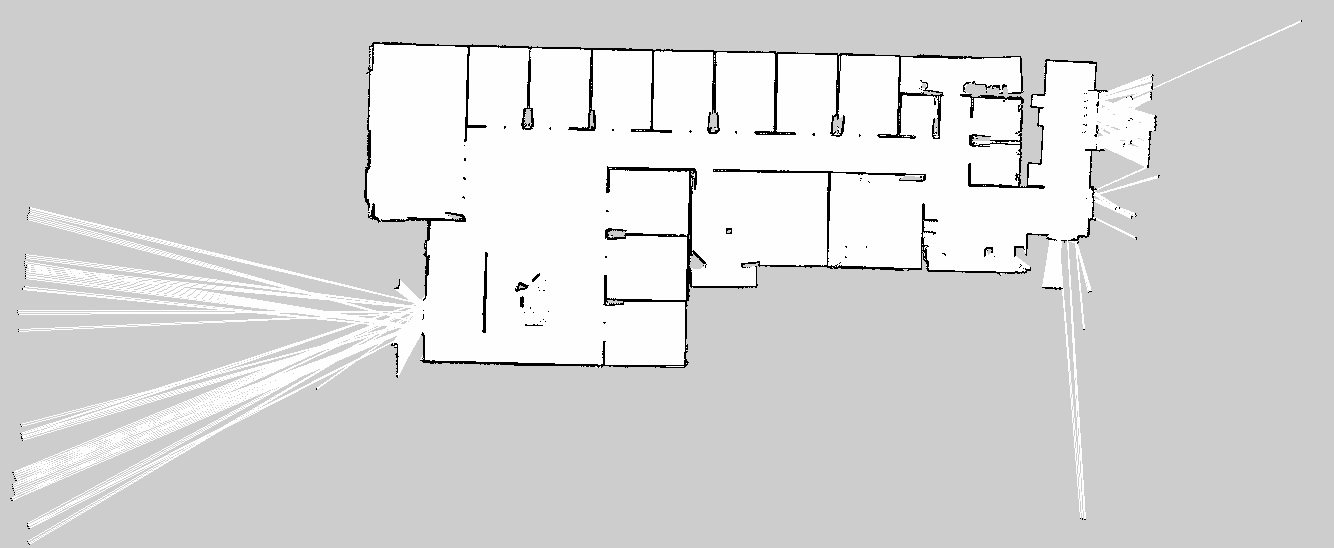
\includegraphics[width=1\textwidth]{images/TRACLabs_scan-clipped.jpg} 

	%{
	%\renewcommand{\thefootnote}{\fnsymbol{footnote}} 
	%\footnotetext{poznámka pod čarou}
	%}

\end{frame}

%%%%%%%%%%%%%%%%%%%%%%%%%%%%%%%% Tvorba polygonu %%%%%%%%%%%%%%%%%%%%%%%%%%%%%%%%%%%%%%%%%%%%%%%%

\section{Tvorba polygonu}
{
\begin{frame}% [plain] % plain znamena, bez standardniho pozadi, ktere maji ostanti slidy
	\frametitle{Tvorba polygonu}

	\begin{itemize}
		\item data ze senzoru ve formě vektoru vzdáleností
		\item výsledný scan $\longrightarrow$ množina bodů vs. polygon
	\end{itemize}

\end{frame}
}

%%%%%%%%%%%%%%%%%%%%%%%%%%%%%%%% Tvorba mapy %%%%%%%%%%%%%%%%%%%%%%%%%%%%%%%%%%%%%%%%%%%%%%%%%%%%

\section{Tvorba mapy}
\begin{frame}
	\frametitle{Tvorba polygonu}

	\begin{columns}[T]
		\begin{column}{0.6\textwidth}
			\begin{itemize}
				\item k dispozici polygon ze senzorického měření \\
				\item booleovské operace nad polygony \\
				\item využití knihovny pro práci s~polygony:
					Clipper 4.6.3 -- an~open source polygon clipping library
					\cite{ClipperLib}
			\end{itemize}
		\end{column}
		\begin{column}{0.4\textwidth}
			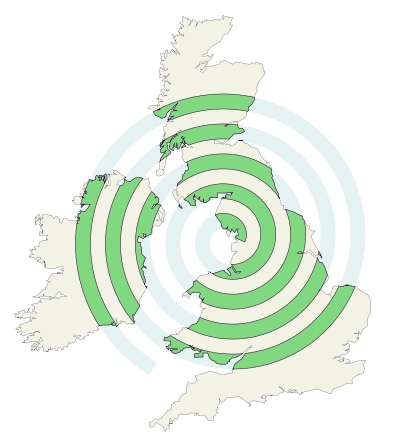
\includegraphics[width=1\textwidth]{images/clipper.png} 
		\end{column}
	\end{columns}

\end{frame}
%%%%%%%%%%%%%%%%%%%%%%%%%%%%%%%% Voroného diagram %%%%%%%%%%%%%%%%%%%%%%%%%%%%%%%%%%%%%%%%%%%%%%%

\section{Voroného diagram}
\begin{frame}
	\frametitle{Voroného diagram z polygonální mapy}

	\begin{columns}[T]
		\begin{column}{0.5\textwidth}
			\vskip 2ex
			\emph{Vstupem} je polygonální mapa $\mathcal S$

			\vskip 2ex

			\pause

			\emph{Clearance radius} bodu $p$ vzhledem k $\mathcal S$ je
			vzdálenost k nejbližšímu bodu množiny $\mathcal S$
			$$\mathsf{d}(p,\mathcal{S}).$$

			\vskip 1ex

			\pause

			\emph{Clearance disc} bodu $p$ je kruh s poloměrem
			$\mathsf{d}(p,\mathcal{S})$ a středem $p$.
				$$ \mathsf{cd}(p,\mathcal{S}) $$

			\vskip 1ex

			\pause \pause \pause \pause \pause

			\emph{Voroného diagram} množiny bodů

		\end{column}
		\begin{column}{0.5\textwidth}
			\includegraphics<1>[width=1\textwidth,clip=true,trim=147pt 165pt 289pt 502pt]{images/01-vd-empty.pdf}
			\includegraphics<2>[width=1\textwidth,clip=true,trim=147pt 165pt 289pt 502pt]{images/02-vd-point.pdf}
			\includegraphics<3>[width=1\textwidth,clip=true,trim=147pt 165pt 289pt 502pt]{images/03-vd-point_with_disk.pdf}
			\includegraphics<4>[width=1\textwidth,clip=true,trim=147pt 165pt 289pt 502pt]{images/04-point_2.pdf}
			\includegraphics<5>[width=1\textwidth,clip=true,trim=147pt 165pt 289pt 502pt]{images/05-point_3.pdf}
			\includegraphics<6>[width=1\textwidth,clip=true,trim=147pt 165pt 289pt 502pt]{images/06-point_4.pdf}
			\includegraphics<7>[width=1\textwidth,clip=true,trim=147pt 165pt 289pt 502pt]{images/07-point_5.pdf}
			\hyperlink{VDdetail}{\includegraphics<8>[width=1\textwidth,clip=true,trim=147pt 165pt 289pt 502pt]{images/08-vd.pdf}}
			\includegraphics<9>[width=1\textwidth,clip=true,trim=147pt 165pt 289pt 502pt]{images/09-wmat.pdf}
		\end{column}
	\end{columns}

	\color{blue}{
	$$ \mathcal{VD}(\mathcal{S}) =
		\left\{ p \in \mathbb{E}^2 \ | \ 
		\mathsf{cd}(p) \text{ se dotýká alespoň dvou různých}\ s \in \mathcal{S} \right\}
	$$}

	\pause
\end{frame}

%%%%%%%%%%%%%%%%%%%%%%%%%%%%%%%% Název sekce %%%%%%%%%%%%%%%%%%%%%%%%%%%%%%%%%%%%%%%%%%%%%%%%%%%%

\begin{frame}
	\frametitle{Vroni}

	Pro konstrukci Voroného diagramů jsme použili kód Vroni \cite{VroniCode}, \cite{Held200195}.

\end{frame}

%%%%%%%%%%%%%%%%%%%%%%%%%%%%%%%% Název sekce %%%%%%%%%%%%%%%%%%%%%%%%%%%%%%%%%%%%%%%%%%%%%%%%%%%%

\section{Využití skeletonu}
\begin{frame}
	\frametitle{Využití topologické kostry - segmentace mapy}

	\begin{itemize}
		\item s topologickou kostrou pracujeme jako s grafem tvořeným
			uzly Voroného diagramu a jeho hranami
		\item v grafu hledáme \emph{kritické uzly}, které tvoří rozhraní
			mezi hledanými segmenty mapy
	\end{itemize}
	\begin{block}{Vlastnosti kritického uzlu $n_c$ podle \cite{Wurm2008Coordinated}}
		\begin{itemize}
			\item stupeň kritického uzlu $\mathsf{deg}(n_c) = 2$
			\item $\exists$ soused $n_i$ kritického uzlu $n_c$ takový, že $\mathsf{deg}(n_i) = 3$
			\item clearance radius kritického uzlu $\mathsf{d}(n_c,\mathcal{S})$ tvoří minimum,
				sousední uzly mají clearance radius větší
			\item kritické uzly spojují už prozkoumané oblasti s neprozkoumanými
		\end{itemize}
	\end{block}

\end{frame}

%%%%%%%%%%%%%%%%%%%%%%%%%%%%%%%% Závěr %%%%%%%%%%%%%%%%%%%%%%%%%%%%%%%%%%%%%%%%%%%%%%%%%%%%%%%%%%

\section{Závěr}
\begin{frame}
	\frametitle{Závěr}

	\begin{block}{Zhodnocení:}
		\begin{itemize}
			\item body k tomu, co by šlo udělat lépe, ehm
		\end{itemize}
	\end{block}
	\begin{block}{Další kroky:}
		\begin{itemize}
			\item upravit Vroni tak, aby umožnilo přenést ze vstupní mapy
				do výsledného grafu informaci o \emph{frontierech}
			\item vyřešit problém s \uv{vnitřkem a nějškem} (jak to formulovat?)
			\item realizovat hledání kritických uzlů
		\end{itemize}
	\end{block}

\end{frame}

\section{Reference}
\begin{frame}
	% tohle byl pokus zahrnout odkaz na video, ale byly s tím spíš problémy
	% \frametitle{\movie[externalviewer]{Závěr}{robojizda.avi}}
	\frametitle{Závěr}

	% The Bibliography
	%\bibliographystyle{plain_cz}
	%\bibliographystyle{czechiso}
	\bibliographystyle{ieeetr}
	\bibliography{bibliography}
	
\end{frame}

%%%%%%%%%%%%%%%%%%%%%%%%%%%%%%%% Dodatek %%%%%%%%%%%%%%%%%%%%%%%%%%%%%%%%%%%%%%%%%%%%%%%%%%%%%%%%

\begin{frame}[label=VDdetail]
	\frametitle{Reprezentace úsečky při konstrukci VD}
	
\includegraphics[height=1\textheight,clip=true,trim=150pt 167pt 409pt 642pt]{images/line_segment-01-endpoint_and_rest_of_line.pdf} 
\end{frame}
\begin{frame}[label=VDdetail]
	\frametitle{Reprezentace úsečky při konstrukci VD}
	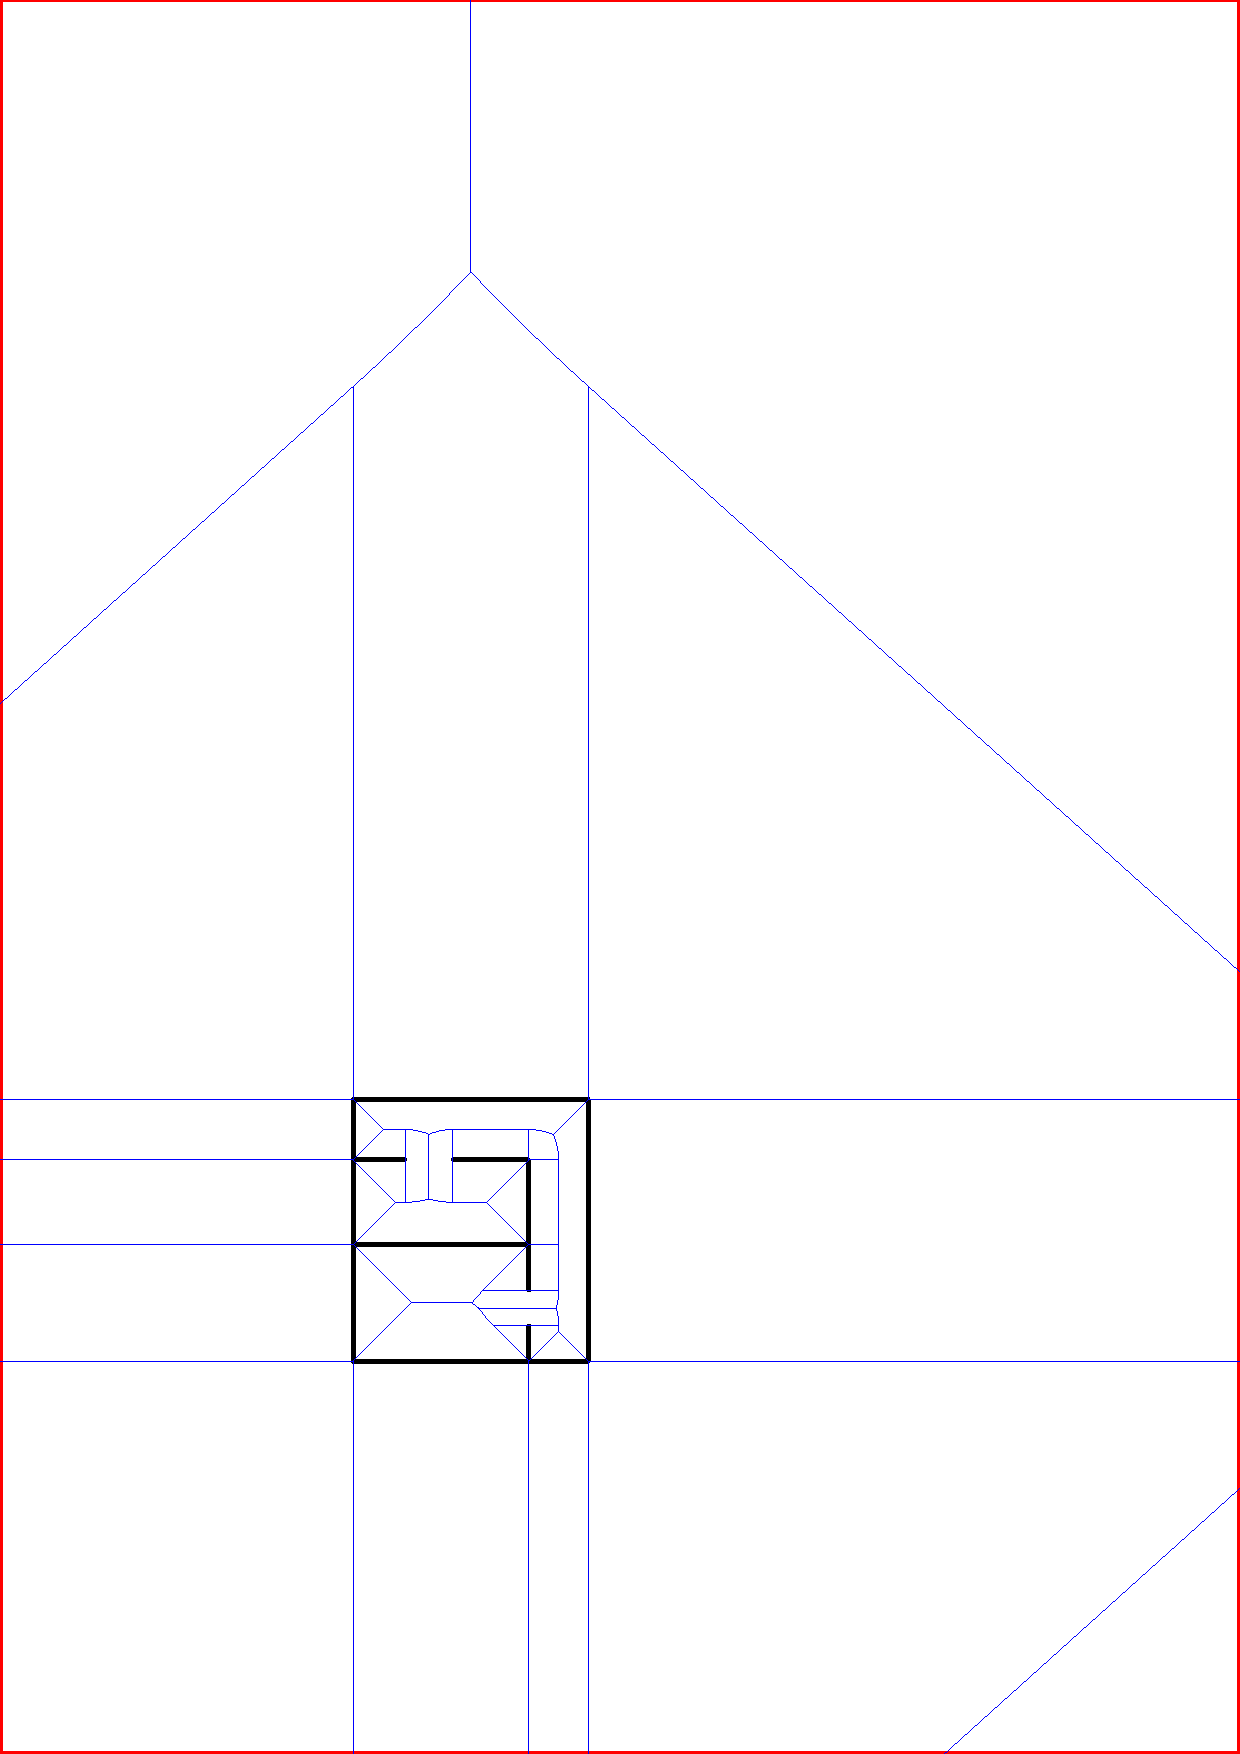
\includegraphics[height=1\textheight,clip=true,trim=150pt 167pt 409pt 642pt]{images/line_segment-02-corner_detail.pdf} 
\end{frame}



\end{document}

